% !TEX encoding = UTF-8
% !TEX TS-program = pdflatex
% !TEX root = ../Tesi.tex
% !TEX spellcheck = it-IT

%************************************************

%************************************************
Il sistema Url2vec si propone come valida alternativa alle metodologie di clustering di siti web basate sul contenuto testuale delle pagine~\cite{Rajaraman11}. A dispetto della diversità delle pagine web nella rete, quelle che risiedono all'interno di una particolare organizzazione, spesso, condividono una certa struttura.
Ad esempio, il sito web di un dipartimento di informatica conterrà pagine riguardante il personale, gli studenti, i corsi, la ricerca che saranno catalogate secondo determinati criteri. Saper sfruttare tale struttura può agevolare notevolmente i task di web mining. Esso infatti aggiunge ulteriore informazione, in modo da estrarre conoscenza strutturata e facilmente processabile. In questa tesi sono state realizzate tre macro componenti.
\begin{itemize}
\item Crawling delle pagine web. Questo è regolato da alcuni parametri che rendono il processo flessibile e altamente modificabile.
\item Costruzione del dataset, ovvero la strutturazione delle informazioni ottenute nel processo precedente, secondo alcuni criteri necessari per le successive elaborazioni.
\item Estrazione di informazione e clustering delle pagine web attraverso la combinazione dell'analisi del contenuto testuale e tecniche di word embedding.
\end{itemize}

Nelle sottosezioni che seguono si descrive il sistema esistente e le tecniche e gli algoritmi utilizzati per la realizzazione degli obiettivi preposti.

\section{Web Crawling per l'estrazione dei dati}
\label{crawling}
Le proprietà che caratterizzano le pagine Web rendono complicato il processo di estrazione di informazioni, soprattutto nel caso in cui i contenuti vengono generati dinamicamente o quando le pagine vengono create o eliminate spesso.

Un Web crawler, chiamato anche web spider o web robot, è un componente software. I suoi obiettivi principali sono:
\begin{itemize}
\item raccogliere il più velocemente ed efficientemente possibile pagine utili, insieme alla struttura ad hyperlink che le collega;
\item aggiornare i contenuti o gli indici dei contenuti di siti Web;
\item copiare tutte le pagine che visita per elaborazioni future, per poi indicizzarle cosi che gli utenti possano trovarle più velocemente;
\item validare gli hyperlink e il codice HTML;
\item eseguire il Web scraping.
\end{itemize}

\begin{figure}[htb]
	\centering
	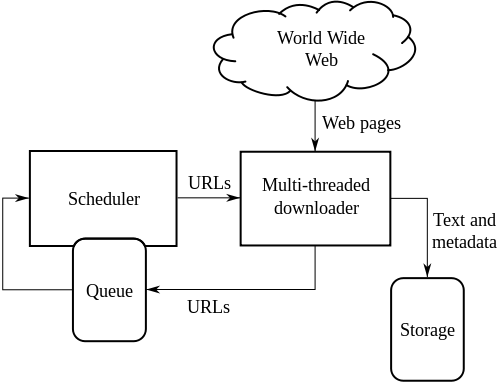
\includegraphics[width = 100mm]{crawlerarch.png}
	\caption{Architettura di un web crawler}
	\label{crawlerarch}
\end{figure}
Esso esplora una pagina alla volta, analizandone la struttura e gli hyperlink contenuti. Questi sono immagazzinati nella ''frontiera'' che inizialmente vuota, conserva tutte le pagine ancora da esplorare. L'ordine di esplorazione e le politiche di filtraggio degli hyperlink possono variare in base al risultato desiderato. 

\subsection{Proprietà del web crawler}
Nel processo di crawling, data la natura non strutturata del web, è necessaria l'applicazione di numerose tecniche e metodologie per un corretto funzionamento.

\subsubsection{Normalizzazione degli URL}
Il termine di normalizzazione, chiamato anche canonicalizzazione di URL, si riferisce al processo di modifica e standardizzazione di un URL in una maniera consistente, ad esempio alcuni siti Web mettono a disposizione gli stessi file o i medesimi contenuti attraverso URL differenti. 
\\\\
\texttt{http://domain.com/products/page.php?product=smartphone}
\\
\texttt{http://domain.com/products/smartphone.php}
\\\\
\texttt{http://www.domain.edu/courses}
\\
\texttt{http://www.domain.edu/courses/index.html}
\\\\
Le due coppie di URL nell’esempio puntano agli stessi contenuti. Altri casi sono URL che differscono solo per il protocollo (''\texttt{http://}'' o ''\texttt{https://}'') o l'omissione della stringa ''\texttt{www}''. Effettuando la normalizzazione, si sceglie un URL come formato di riferimento per accedere ad un determinato contenuto. Ci sono diversi tipi di normalizzazione che possono essere usati, come la conversione in minuscolo, rimuovere i ''.'' e ''..'' portando gli URL relativi ad URL assoluti, aggiungere slash finali al componente di percorso non vuoto.
\\\\
Una soluzione consiste nella creazione di un dizionario che ha come chiavi gli hashcode del contenuto testuale delle pagine e come valori una lista di tutti i diversi URL che hanno quel contenuto. In questo modo si riduce il problema ad una sola operazione così da annullare le relazioni e i vari di pattern da scovare nall'analisi degli URL per capire se sono la stessa pagina o meno. 

\subsubsection{Ricerca all'interno dello stesso dominio}
Per estrarre informazione e per il successivo processo di clustering delle pagine web, è necessario che le pagine estratte si riferiscano allo stesso dominio, o in altri termini, che appartengano allo stesso sito web.
\\
Questo viene effettuato per sfruttare la struttura gerarchica del dito web rivolto principalmente riuscire a  raccogliere le informazioni nascoste nel grafo e sopratutto negli hyperlink.

\subsubsection{Dimensione della ricerca}
Anche limitando la ricerca ad un solo dominio, la dimensione delle pagine da esplorare, e quindi la grandezza della frontiera, può aumentare considerevolmente o addirittura portare il processo di crawling a divergere.

\begin{figure}[htb]
	\centering
	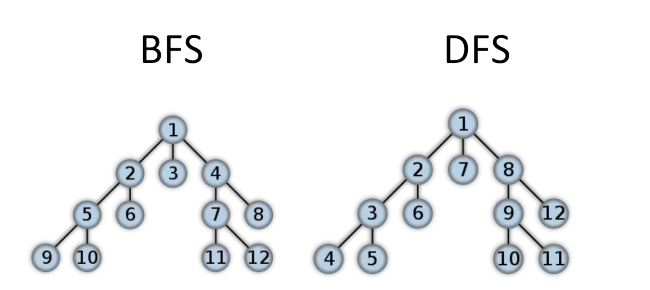
\includegraphics[width = 100mm]{breadthdepth.png}
	\caption{Differenze tra ricerca in ampiezza e ricerca in profondità}
	\label{breadthsearch}
\end{figure}

È stata utilizzata una ricerca in ampiezza con un limite variabile di profondità. Ponendo un limite all'esplorazione del grafo delle pagine si garantisce la la terminazione del processo di crawling e utilizzando una ricerca in ampiezza si dà priorità alle pagine vicine al nodo radice (comunemente l'homepage). Questa scelta è stata dettata anche dal cercare di evitare le cosiddette ''spider traps''. Queste sono dei meccanismi utilizzati, intenzionalmente o involontariamente, dai server oggetto di crawling, che possono portare ad una generazione dinamica e potenzialmente infinita in URL univoci, e quindi considerati come pagine diverse. Questo può essere evitato non aggiungendo alla frontiera URL che contengono il carattere ''?'', ma questo non è sempre efficace.
\\\\
Inoltre è stato osservato che nei siti web entity-oriented, le informazioni ricercate si trovano quasi sempre nei primi livelli di gerarchia \cite{He13}.

\subsubsection{Restrizione dell'esplorazione}
La restrizione può essere effettuata sulle pagine da esplorare o dalla frequenza di richieste che è possibile effettuare.
\\\\
Il robots exclusion protocol è uno standard che consiste in un file (robots.txt), posto alla radice della gerarchia di un sito Web. In pratica, il file indica le regole utilizzate dai crawler per applicare restrizioni di analisi sulle pagine di un sito web. 
\\\\
Molte volte i crawler non sono ben accetti, in quanto possono rallentare pesantemente la navigazione. Se server effettua dei controlli sulle richieste ricevute e queste hanno una frequenza troppo elevata o seguono uno schema riconducibile ad una macchina queste possono essere ignorate. Può capitare che richieste continue e non curanti delle restrizioni imposte portino a bandire l'indirizzo IP del servizio trasgressore.\\
Per evitare tali conseguenze è opportuno seguire una certa etica nell'operazione di crawling.

\subsection{Estrazione delle liste}
Riuscire a strutturare dati non strutturati può rivelarsi ostico. Molti tentativi, più o meno efficaci, sono stati effettuati a tale proposito.
\\
In questa tesi uno degli obiettivi è stato quello di prendere in considerazione i collegamenti all'interno delle pagine web, seguendo i percorsi generati dalla concatenazione di più hyperlink. Questa scelta è stata effettuata sulla base dei recenti progressi nel campo del natural language processing (NLP)~\cite{Turian10}. Esplorando la struttura del grafo del web, data la forte connessione che esiste fra i suoi nodi, estrarre informazione può rivelarsi un operazione tutt'altro che banale. 
\\\\
È stato introdotto il concetto di \textbf{lista}. 
Per permettere una migliore visualizzazione dell’informazione descritta, quasi tutte le pagine web vengono formattate utilizzando regole CSS. Di conseguenza, per poter effettuare correttamente questo task, bisogna prima elaborare la pagina Web con tutte le informazioni grafiche sui nodi HTML e solo successivamente si può procedere alla loro estrazione. Grazie alle informazioni ricavate dall’HTML della pagina Web e dalla posizione e dimensione dei singoli nodi, è possibile stabilire una struttura gerarchica ad albero dei nodi che la compongono. Questa struttura gerarchica ad albero permette di scoprire i record, ovvero dati strutturati (ad esempio provenienti da database) che sono allineati orizzontalmente, verticalmente e anche strutturalmente (elementi HTML ul, li, . . . ); permette quindi di individuare dei gruppi di record, ovvero delle liste di record.
\\
L’individuazione delle liste di raggiungere pagine che contengono elementi simili a quelli contenuti nella pagina che si sta visualizzando. 
In questo modo le pagine dovrebbero essere accessibili solo attraverso percorsi predeterminati e non in maniera fortemente connessa. I nodi e gli archi risultanti risultano così un sottoinsieme di quelli originali.

\section{Costruzione del dataset}
I dati estratti nel processo vanno organizzati e ampliati in modo da garantire l'accesso e l'elaborazione in maniera agevole.
\\
Il processo di crawling restituisce il grafo delle pagine web e il contenuto testuale di ogni pagina esplorata a queste va aggiunta la generazione delle sequenze. Inoltre per un minor spreco di risorse si è optato per la conversione degli URL in codici, ovvero una associazione univoca fra un URL e un codice (e.g. un numero) molto più corto, così da risparmiare tempo di elaborazione e spazio di archiviazione. Segue una analisi sul processo di generazione delle sequenze.


\subsection{Generazione delle sequenze}
Le sequenze rappresentano un percorso che un attraversatore casuale della rete seguirebbe cliccando su un hyperlink a caso fra tutti quelli disponibili nella pagina corrente (o eventualmente nelle liste). Questi percorsi, chiamati \textbf{random walk} (o passeggiate aleatorie), sono stati largamente utilizzati in molti algoritmi sui grafi e sul web~\cite{aldous14} in quanto buone approssimazioni di comportamenti casuali. Il problema di questa tecnica applicata al web si presenta quando l'attraversatore casuale arriva ad una pagina priva di hyperlink. La soluzione più diffusa consiste nell'effettuare un ''salto'' verso una qualsiasi altra pagina quando non ci sono outlink da seguire. 
\\\\
Qui il problema non si pone, in quanto le sequenze generate hanno una lunghezza fissata prima dell'esecuzione e se la generazione dovesse bloccarsi, la sequenza risultante sarà solo più piccola. Questa scelta è dovuta dal fatto che l'informazione cercata scaturisce da percorsi reali di navigazione e non necessita una lunghezza obbligatoria da rispettare, in quanto le sequenze possono essere viste come frasi di un testo, dove le parole sono gli URL.
\\\\
Per motivi di sperimentazione sono stati implementati tre tipi diversi di random walk, utilizzabili modificando i parametri di esecuzione dell'algoritmo.

\subsubsection{Random Walk}
Questo è il caso standard, ovvero si parte da un nodo casuale del grafo e si segue ogni volta un arco a caso fra quelli disponibili, fino al raggiungimento della lunghezza prefissata o all'impossibilità di proseguire.
\\
Da notare che questo processo e il precedente non sono completamente separati, in quanto la scelta di un nodo casuale e la consecutiva traiettoria, possono portare all'esplorazione di pagine non precedentemente visitate. È quindi necessario mantenere aggiornato il grafo immagazzinato.
\begin{figure}[htb]
	\centering
	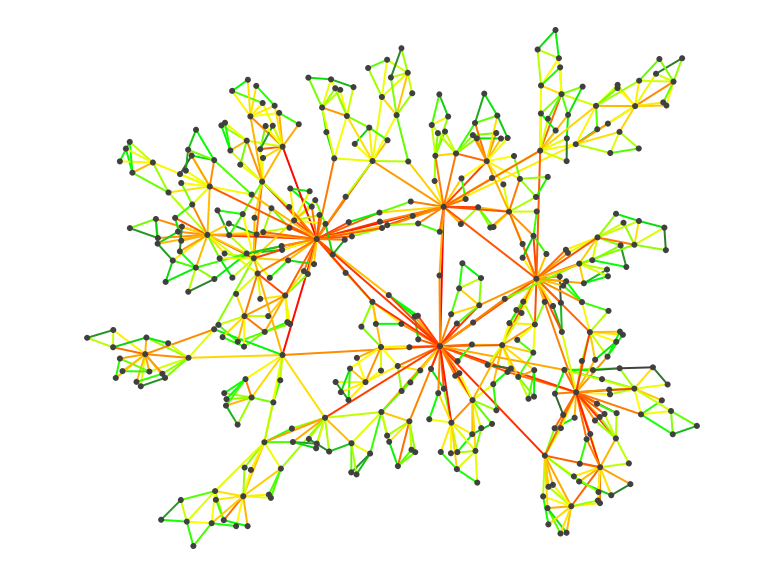
\includegraphics[width = 100mm]{randomWalkongraph.png}
	\caption{Random walk sul grafo. }
	\label{englishchinese}
\end{figure}
\subsubsection{Random Walk con partenza fissa}
Qui l'unica differenza consiste nel punto di partenza del cammino. Infatti si può partire in un nodo prefissato del grafo (generalemnte l'homepage di un sto web), in modo da esplorare più percorsi possibili avente quel nodo come origine.

\subsubsection{Random Walk attraverso le Liste}
Qui invece si può seguire uno dei due approcci precedenti, ma con il vincolo delle liste, quindi limitando la camminata ad un sottoinsieme di quella precedente.

\begin{algorithm}[H]
\caption{Crawling BFS}
\begin{algorithmic}

	\State $url\gets homepage$;	\Comment{Pagina da cui iniziare}
	\State $queue\gets empty$ \Comment{Coda per la BFS}
	\State $analyzedVertex.add(url)$;	\Comment{Insieme di url già visitati}
	\State $maxDepth url$;	\Comment{Massima profondità di esplorazione}
 	
 	\vspace*{+0.5cm}
 	
	\State \textbf{Begin}
	\While{$queue \neq empty$} 
		\State $urlToAnalyze\gets queue.dequeue()$
		
		\If{$urlToAnalyze.depth \leq maxDepth$}
			\State $outlinks \gets urlToAnalyze.getOutlinks()$
		\Else
			\State $urlToAnalyze$
		\EndIf
		\If{$outlinks \neq null$}
			\State $outlinks \gets urlToAnalyze.getOutlinks()$
			\State $analyzedVertex.add(outlinks)$
			\State $serialize(urlToAnalyze)$
			\For{\textbf{each} link in outlinks}
				\State $serialize(link)$
				\State $queue.enqueue(link, urlToAnalyze + 1)$
			\EndFor
		\EndIf
		
	\EndWhile
	\State \textbf{End}
\end{algorithmic}
\end{algorithm}

\begin{algorithm}[H]
\caption{Generazione delle sequenze}
\begin{algorithmic}

	\State $numRandomWalks$;	\Comment{Numero di Random Walk da generare}
	\State $lengthRandomWalks$ \Comment{Lunghezza dei Random Walk}
 	
 	\vspace*{+0.5cm}
 	
	\State \textbf{Begin}
	\State $node \gets \Call{randomnode}{}$
	\For{$i \gets 0 \to numRandomWalks$} 
		\State $sequence.add(node)$
		
		\While{$sequence.length \leq lengthRandomWalks$}
			\If{$node.hasOutlinks()$}
				\State $node \gets node.getOutlinks(RandomIndex)$
				\State $sequence.add(node)$
			\Else
				\State $break$
			\EndIf
		\EndWhile
		\State $serialize(sequence)$
		
	\EndFor
	\State \textbf{End}
\end{algorithmic}
\end{algorithm}

\section{Clustering delle pagine web}
In questa sezione si parlerà della soluzione proposta come alternativa alle normali tecniche di clustering delle pagine web basate esclusivamente sul contenuto testuale. Infatti il fulcro del sistema è basato su metodologie nate nel campo del \textbf{Natural Language Processing} ma applicate nel contesto web, in modo da aggiungere ulteriore informazione utile. Qui sarà approfondita l'idea alla base del lavoro svolto e le diverse opzioni che l'algoritmo mette a disposizione. 
L'algoritmo prende in input il grafo di un sito web ele sequenze di random walk generate restituisce rappresentazioni vettoriali per ogni pagina.
La fase di sperimentazione vera e propria sarà approfondita nel capitolo successivo.

\subsection{NLP nel web: URL embedding}
I recenti algoritmi di word embedding, riescono a tenere in considerazione sempre più fattori e quindi restituire vettori sempre più accurati. In particolare vengono incluse informazioni riguardanti il contesto di una parola, ovvero le altre parole che sono contenute all'interno delle frasi in cui compare quella sotto esame. Questa informazione riesce ad estrarre correlazioni nascoste e raggruppare i termini in classi. Può sembrare banale ma diversamente dal text clustering tradizionale, dove le parole vengono considerate al livello di documento, qui vengono considerate a livello di frase. Un esempio può riguardare il controverso caso delle analogie. 
\\\\
È stato osservato che correlazioni nascoste possono trovarsi nella differenza tra coppie di vettori~\cite{Mikolov13}, come nel caso di parole simili ma con leggere differenze come il genere o il numero, infatti esse appaiono in frasi tendenzialmente identiche, ma con delle piccole differenze. In questo caso l'informazione può essere interpretata come il genere o il numero.
\\\\
Informazioni simili possono essere trovate anche nel campo del web, analizzando i percorsi di URL come se fossero frasi. È ormai consolidata la questione dell'autorità di alcune pagine~\cite{Kleinberg99}
e di come queste abbiano un maggior numero di link in entrata. Alcune pagine tuttavia saranno accessibili prevalentemente attraverso alcuni percorsi e si troveranno quindi in un contesto con elementi simili. Il problema adesso è riuscire a dare un senso a queste correlazioni e dargli un significato utilizzabile. Nello sviluppo di Url2vec tuttavia sono emerse corrispondenze abbastanza naturali, come le pagine dei professori con i relativi corsi insegnati o i laboratori di afferenza. Queste relazioni sono dovute al fatto che il grafo di un sito web è fortemente connesso, ma la maggior parte delle volte in cui appare un determinato corso di studio appare anche il relativo docente e viceversa. 

\subsection{Differenza tra parole ed URL}
La sola analisi delle sequenze comunque può risultare limitata. Gli URL non sono parole, in quanto ad essi è associata ulteriore informazione, ovvero il contenuto testuale. Questa proprietà si è rilevata molto utile, infatti combinando le informazioni ricavate esaminando tutti e due gli aspetti, il grado di accuratezza del processo di clustering è salito in modo significativo. 

